
%-[Phần mở đầu chương
\chapter[HƯỚNG DẪN VIẾT LUẬN ÁN BẰNG \LaTeX]{HƯỚNG DẪN\\ VIẾT LUẬN ÁN BẰNG \LaTeX} \label{chchukytapthedathanhphan}%
%\minitoc %
%\setcounter{baitap}{0}
%\thispagestyle{empty}
%\vspace*{1cm}
%]-
 
\textbf{Chương này là phần trọng tâm của Luận án, bao gồm: phần cài đặt môi trường và gói phần mềm vietkey.luanan.1.2.cls, tiếp theo là phần hướng dẫn sử dụng gói phần mềm này, cuối cùng là một số lưu ý khi sử dụng \LaTeX\ trong việc soạn thảo luận án.}

\section{\bf Cài đặt môi trường soạn thảo \LaTeX} \label{mucchkydatp}

\subsection{Cài đặt \LaTeX}
\begin{itemize}
	\item Cài đặt lõi cho môi trường \LaTeX\ : vào trang chủ https://miktex.org/ và download phần mềm MiKTeX tương ứng cho hệ điều hành đang sử dụng. Không nên cài gói này từ các link hay đĩa CD không chính chủ.
	\item Nên cài đặt phần mềm soạn thảo \LaTeX\ là TeXStudio từ trang chủ   http://www.texstudio.org/ (mặc dù trong bộ MiKTeX cũng đã có kèm phần mềm soạn thảo là TeXworks nhưng phần mềm này khá thô sơ và ít tính năng nâng cao).
\end{itemize}

\subsection{Cài đặt vietkey.luanan.1.2.cls}
\begin{itemize}
	\item Vào trang web theo đường dẫn \textbf{http://j.mp/trinhbayluanan} và download file \textbf{MauLA.zip}.
	\item Copy  và giải nén file\textbf{MauLA.zip} vào thư mục làm việc, là thư mục chứa file .tex gốc của luận án, luận văn.
\end{itemize}

\subsection{Các file tối thiểu của gói vietkey.luanan}
\begin{tcolorbox}
\begin{itemize}
	\item \textbf{vietkey.luanan.1.2.cls}
	\item \textbf{luanan.bbx}
	\item \textbf{clean.bat}
\end{itemize}
\end{tcolorbox}

\section{\bf Hướng dẫn soạn thảo luận án bằng \LaTeX} \label{mucchkydatp}

Cách đơn giản nhất là sử dụng class của tác giả đã xây dựng là \textit{vietkey.luanan} phiên bản hiện thời là 1.2 (25/8/2017).

File gốc hay master là \textbf{LuanAn.tex} xem Hình \ref{h.goc}. Các chương mục sẽ được cấu trúc thành các file khác nhau. 
Dùng lệnh \textbf{\textbackslash include\{tenFile.tex\}} để gắn các chương mục này vào file gốc. Các file này có thể nằm ở thư mục khác nhưng để tiện soạn thảo các chương mục này nên nằm trong cùng một thư mục.

Các lệnh do tác giả xây dựng có tiết đầu tố là \textbf{\textbackslash VK*}.

\begin{figure}[!ht]	
	\begin{center}		
		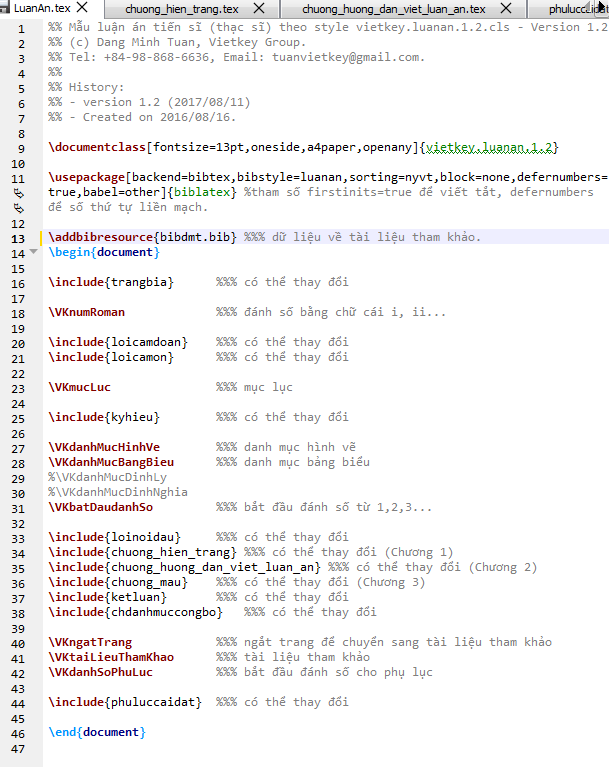
\includegraphics[scale=1.0]{master}
		\\		
	\end{center}	
	\caption{File gốc LuanAn.tex}	
	\label{h.goc}
\end{figure}

\subsection{Tài liệu tham khảo}

Ví dụ tham chiếu tài liệu tham khảo \cite{V10948}, hay \cite{V10944}, hoặc \cite{S10950}, và một số khác nữa: \cite{S9619}, \cite{S10950}. \cite{S10949}, \cite{S10791}, \cite{S10541}. \cite{S10921}, \cite{S556}, \cite{K02}.

Nhập liệu về tài liệu tham khảo trong file .bib như thường lệ xem file mẫu \textit{bibdmt.bib} đi kèm , tuy nhiên để có thể phân loại tài liệu tiếng Việt và tiếng Anh, chúng ta thêm hai trường là \textbf{langid = \{slovene\}} và \textbf{keywords = ``Vietnam''} để phân biệt với các văn bản tiếng Anh, có thể làm tương tự với tiếng Nga, tiếng Trung. \textit{Đáng tiếc là gói BibLaTex chưa hỗ trợ ngôn ngữ tiếng Việt do đó tác giả phải chọn ngôn ngữ \textit{slovene}} để tùy biến.

Ngoài ra ở trong file .bib có thể gõ tiếng Việt Unicode. Dưới đây là một mục (bài báo) trong file .bib có số liệu bằng tiếng Việt.
%\begin{lstlisting}[frame=trBL][language=TeX]{}

\textbf{Bài báo:}

\begin{tcolorbox}
\begin{verbatim}
@article{Bai22,
author    ="Nguyễn Hiếu Minh and Đỗ Thị Bắc",
title     ="{Một số lược đồ chữ ký số mù mới 
            dựa trên bài toán DLP và ECDLP}",
journal   ="Tạp Chí Khoa học và Công nghệ năm 2015",
volume    ="11",
number    ="5",
pages     ="3--11", 
year      ="2015",
langid    = {slovene},
keywords  = "Vietnam"
\end{verbatim}
\end{tcolorbox}

%\end{lstlisting}

\textbf{Sách:}

\begin{tcolorbox}
\begin{verbatim}
@book{V10945,
author ="Lưu Hồng Dũng",
title  ="Nghiên cứu, phát triển các lược đồ chữ ký số tập thể",
publisher ="Luận án tiến sĩ kỹ thuật, Học viện KTQS",
year ="2013",
keywords ="Vietnam"
\end{verbatim}
\end{tcolorbox}

\section{\bf Các gói đã được nhúng trong \textit{vietkey.luanan}}

\begin{itemize}
	\item \textbackslash usepackage[vietnam]\{babel\}
	\item \textbackslash usepackage[utf8]\{vietnam\}
	\item \textbackslash usepackage\{enumerate\}
	\item \textbackslash usepackage\{amsmath,amsxtra,amssymb,latexsym, amscd,amsthm\}
	\item \textbackslash usepackage\{indentfirst\}
	\item \textbackslash usepackage\{mathptmx\}
	\item \textbackslash usepackage\{fancyhdr\}
	\item \textbackslash usepackage\{picinpar\}
	\item \textbackslash usepackage\{floatflt\}
	\item \textbackslash usepackage\{epic\}
	\item \textbackslash usepackage\{curves\}
	\item \textbackslash usepackage\{makeidx\}
	\item \textbackslash usepackage\{longtable\}
	\item \textbackslash usepackage\{multicol\}
	\item \textbackslash usepackage\{listings\}
	\item \textbackslash usepackage[fontsize=13pt]\{scrextend\}
	\item \textbackslash usepackage[tight,vietnam]\{minitoc\}
	\item \textbackslash usepackage\{fancybox\}
	\item \textbackslash usepackage\{pdflscape\}
	\item \textbackslash usepackage\{tcolorbox\}
	\item \textbackslash usepackage\{enumitem\}  
	\item \textbackslash usepackage\{tikz\}
	\item \textbackslash usepackage[utf8]\{inputenc, vietnam\}
	\item \textbackslash usepackage\{color, graphicx\}
	\item \textbackslash usepackage[chapter]\{algorithm\}
	\item \textbackslash usepackage\{algorithmic\}
	\item \textbackslash usepackage\{eso-pic,calc\}
	\item \textbackslash usepackage\{hyperref\}
	\item \textbackslash usepackage\{bookmark\}
	\item \textbackslash usepackage\{titlesec\}
	\item \textbackslash usepackage\{thmtools\}
	\item \textbackslash usepackage\{booktabs\}
	\item \textbackslash usepackage\{geometry\}
	
\end{itemize}

\section{\bf Một số kinh nghiệm và lưu ý khi sử dụng}
\begin{itemize}
	\item Trong một số trường hợp khi cập nhật tài liệu tham khảo, việc đồng bộ giữa tham chiếu tài liệu tham khảo và dữ liệu tài liệu tham khảo có thể có sự khác biệt, khi đó cần phải xóa các file trung gian để phần mềm soạn thảo biên dịch lại từ đầu. Tác giả đã tạo ra một file chạy \textbf{clean.bat} tự động xóa hết các file này. Kích hoạt bằng cách nháy đúp con chuột vào file này trong File Explore.
	\item Tên các chương có thể được hiển thị khác nhau trong phần nội dung và phần mục lục. Trong phần nội dung do phải dùng font lớn để làm tiêu đề chương nên với tên dài cần phải ngắt dòng, tuy nhiên ở phần mục lục dùng font chữ nhỏ hơn nếu để tự động thì ở phần mục lục cũng ngắt dòng tương ứng như vậy sẽ không hợp lý. Để có thể hiển thị và ngắt dòng khác nhau có thể dùng dấu [] và \{\} sau lệnh \textbackslash chapter tương ứng với hiển thị trong mục lục và tiêu đề trong nội dung luận án.
\end{itemize}

\section{\bf Kết luận chương \ref{chchukytapthedathanhphan}}

\LaTeX\ nói chung và gói bilatex đang là xu thế được sử dụng để biên soạn luận án, luận văn và quản lý, sắp xếp tài liệu tham khảo một cách mềm dẻo và linh hoạt. Với class mới được phát triển ``\textbf{vietkey.luanan}'' có thể đáp ứng được hầu hết các yêu cầu trình bày luận án và cách sắp xếp và trích dẫn tài liệu tham khảo do các trường đại học ở Việt Nam quy định.

Mọi góp ý và đóng góp cho tài liệu cũng như gói class ``\textbf{vietkey.luanan}'' xin gửi về \textbf{tuanvietkey@gmail.com} hoặc thông qua \textbf{facebook.com/tuanvietkey}.

